
In this Chapter, we present expected results on nucleon-spin flavor decomposition according various methods described in Chapter 2, and 
the corresponding statistical uncertainties.  We also address major sources of systematical uncertainties.

\section{Systematic uncertainties on asymmetry $A_{1He}^h$ and $A_{1n}^h$}

Knowledge of target polarization and dilution factor dominates the systematic uncertainty of $A_{1n}^h$.
The effects of radiative corrections will be treated in a Monte Carlo simulation
following the procedures of the HERMES analysis~\cite{Airapetian:2004zf}, which found that the 
systematic uncertainties introduced by this procedure are negligible.  
Kinematic smearing will also be treated following the procedure of the HERMES analysis. 

\vspace{5.0mm}
\noindent ~\hspace{0.25cm} ~Major systematic uncertainties on $A_{1He}^h$:  \\
\noindent ~\hspace{0.25cm} ~Target polarization $\delta P_T/P_T$:  \hfill           $\pm 2.5\%$  relative \\ 
\noindent ~\hspace{0.25cm} ~Beam polarization $\delta P_B/P_B$:    \hfill           $\pm 2.0 \%$ relative \\
\noindent ~\hspace{0.25cm} ~Helicity correlated beam charge uncertainty $\delta (Q_+/Q_-)$:   \hfill  $\ll 10^{-4}$ absolute \\
\noindent ~\hspace{0.25cm} ~Radiative correction and kinematic smearing:                \hfill           $\pm 1.5 \%$  relative \\
\noindent ~\hspace{0.25cm} ~Knowledge of $R$ and correction from $A_{\perp}$:                \hfill           $\pm 1.5 \%$  relative \\
\vspace{-3.0mm}
{\bf 
\noindent \hspace{0.5cm} Total systematic uncertainty on $A_{1He}^h$  \hfill          $\pm 3.8 \%$  relative } \\

\vspace{0.0mm}
\noindent ~\hspace{-0.4cm} ~Extra systematic uncertainties involved in extracting $A_{1n}^h$:  \\
\noindent ~\hspace{0.25cm} ~Dilution factor $\delta f/f$:        \hfill           $\pm 2.5 \%$  relative \\
\noindent ~\hspace{0.25cm} ~Effective neutron polarization in $^3$He $\delta P_n/P_n$:  \hfill           $\pm 4.2\%$  relative \\ 
%\noindent ~\hspace{0.25cm} ~$\pi N$ final state interaction:  \hfill           small \\ 
\vspace{-3.0mm}
{\bf 
\noindent \hspace{0.5cm} Systematic uncertainty on $A_{1n}^h$ (exp.+theory):  \hfill          $\pm 6.2 \%$  relative } \\

\section{Expected results from NLO global fit and impacts to DSSV2008}

The high precision SIDIS asymmetry data of this experiment will add strong constraints to quark polarization $\Delta q$ as well as gluon polarization $\Delta g$ through NLO global fit. An independent effort to investigate the impacts of this experiment to DSSV2008, and DSSV2014 global fits is currently under way by Dr. R, Sassot of the  DSSV group.   The results of the impact study will be presented at PAC42 in July 2014,  a paper will be posted on arXiv based on this  study.    

An earlier impact study~\cite{epjcxj2006} of JLab-6GeV $^3$He measurement  to NLO global fit has been conducted based on an expected data set two orders of magnitude smaller than this experiment, corresponding to a BigBite and HRS spectrometer combination.  Even with an equivalent of $\sim 1\%$ data set of this experiment, significant improvements on $\Delta q$ and $\Delta g$ are shown to have a similar constrain power as the RHIC 2006 $A_{LL}^{\pi^0}$ data set~\cite{epjcxj2006}.     

\section{Expected results from Leading-Oder ``purity''  method}
\subsection{Results of ``purity'' method at fixed-$z$ bins}
At each fixed $z$-point corresponding to each $(x,Q^2)$ ,  `purity'' method is applied to solve for $\Delta u/u$, $\Delta d/d$, $\Delta \bar{u}/\bar{u}$,  $\Delta bar{d}/\bar{d}$ and $(\Delta s+\Delta \bar{s})/(s+\bar{s})$ from five measured asymmetries $A_{1n}$, $A_{1n}^{\pi^+}$, $A_{1n}^{\pi^-}$, $A_{1n}^{K^+}$ and  $A_{1n}^{K^-}$.  We note that we have not used  the extra constraints from $A_{1n}^{\pi^0}$ measurement yet, due to the expected  $\sim 10 \%$  $\pi^0$ reconstruction efficiency.

The expected statistical uncertainties of fixed$-z$ ``purity'' spin flavor decomposition are listed in Appendix~\ref{App:spin_flavor}, Table~\ref{tab:purity1}  and Table~\ref{tab:purity2} . For different $z$-bins corresponding to the same $(x,Q^2)$, the $z$-dependency, or the lack of it, of the extracted $\Delta q/q$ can be used to verify the predicted Leading-Order $x-z$ naive separation, or set a systematic upper limit on how well this assumption holds. 

Once the $z$-independence behavior is verified, data from different $z$-bins corresponding to the same $(x,Q^2)$ will add extra independent linear equations to constrain the five unknowns of $\Delta q/q$. The results are listed in Table~\ref{tab:purityallz}. Notice that relative quark polarization  uncertainty values larger than $100 \%$ are not listed in the table.  
%
%-------------------------------------------------------------------------------
\begin{table}[htbp]
\begin{center}
%\vspace{-0.5cm}
\begin{tabular}{|ccc||ccccc|}
\hline
$\langle x \rangle $   & $ \langle Q^2 \rangle $   &  \# of  & $\displaystyle{\delta \left({ \Delta u \over u} \right)}$  & $\displaystyle{\delta \left({ \Delta d \over d} \right)}$&
$\displaystyle{ \delta \left({ \Delta \bar{u} \over\bar{u}} \right)}$ & $\displaystyle{\delta \left({ \Delta \bar{d} \over\bar{d}} \right)}$ &  $\displaystyle{\delta \left({ \Delta s + \Delta  \bar{s} \over s+ \bar{s}} \right)}$  \\
                       & GeV$^2$            &       constrain    &  $\%$  &   $\%$    &  $\%$    &     $\%$    &       $\%$                                                   \\ \hline 
   E$_0$=11 GV  &    & &         &          &         &          &         \\
   0.166 &   3.288 & 25&        0.90 &         0.63 &        18.79 &         1.66 &        12.88 \\
   0.249 &   4.639 & 25&        0.70 &         0.64 &        28.84 &         2.73 &        20.06 \\
   0.347 &   6.090 & 25&        0.86 &         0.98 &        65.77 &         8.73 &        54.18 \\
   0.445 &   7.384 & 25&        1.13 &         1.64 &            - &        30.42 &            - \\
   0.543 &   8.483 & 21&        1.77 &         3.15 &            - &            - &            - \\
   0.641 &   9.583 & 13&        3.92 &         8.74 &            - &            - &            - \\
   E$_0$=8.8 GV  &    & &         &          &         &          &         \\
   0.168 &   2.576 & 25&        0.94 &         0.68 &        20.53 &         1.72 &        13.93 \\
   0.248 &   3.544 & 25&        0.76 &         0.71 &        32.33 &         2.89 &        22.49 \\
   0.345 &   4.610 & 25&        1.04 &         1.16 &        77.42 &        10.18 &        63.44 \\
   0.436 &   5.598 & 21&        1.55 &         2.25 &            - &        40.46 &            - \\
   0.540 &   6.368 & 13&        2.96 &         5.36 &            - &            - &            - \\
 \hline
\end{tabular}
\end{center}
\caption{\label{tab:purityallz}  The expected statistical uncertainties of  all $z$-bins,  according to  `LO `purity' spin flavor decomposition.  Relative quark polarization  uncertainty values larger than $100 \%$ are not listed in the table.
%Values of $x u_v(x)$ and $x d_v(x)$ f are rom CTEQ leading order.
}
\end{table}
%------------------------------------------------------------------------------

The expected statistics of Leading-Order ``purity'' method extracted  $\Delta q/q$, compared with HERMES~\cite{Airapetian:2004zf}  experiment and predictions from Statistical Model,   are  shown in Fig.~\ref{fig:delta5q}.  The COMPASS experiment~\cite{Alekseev:2010ub}  presented its results in $x\cdot \Delta q$ not in ratios. We can clearly pin down $\Delta u/u$ $\Delta d/d$, and $\Delta \bar{d}/\bar{d}$ very well, as expected. We can also obtain reasonable precisions for $\Delta \bar{u}/\bar{u}$ and $\Delta s/s$. Of course, when combined with future proton (NH$_3$) target data from CLAS12,  precision on $\Delta \bar{u}/\bar{u}$ can be much improved.
%---------------------------------------------------------------------------------------------
\begin{figure}[htbp]
\centering
    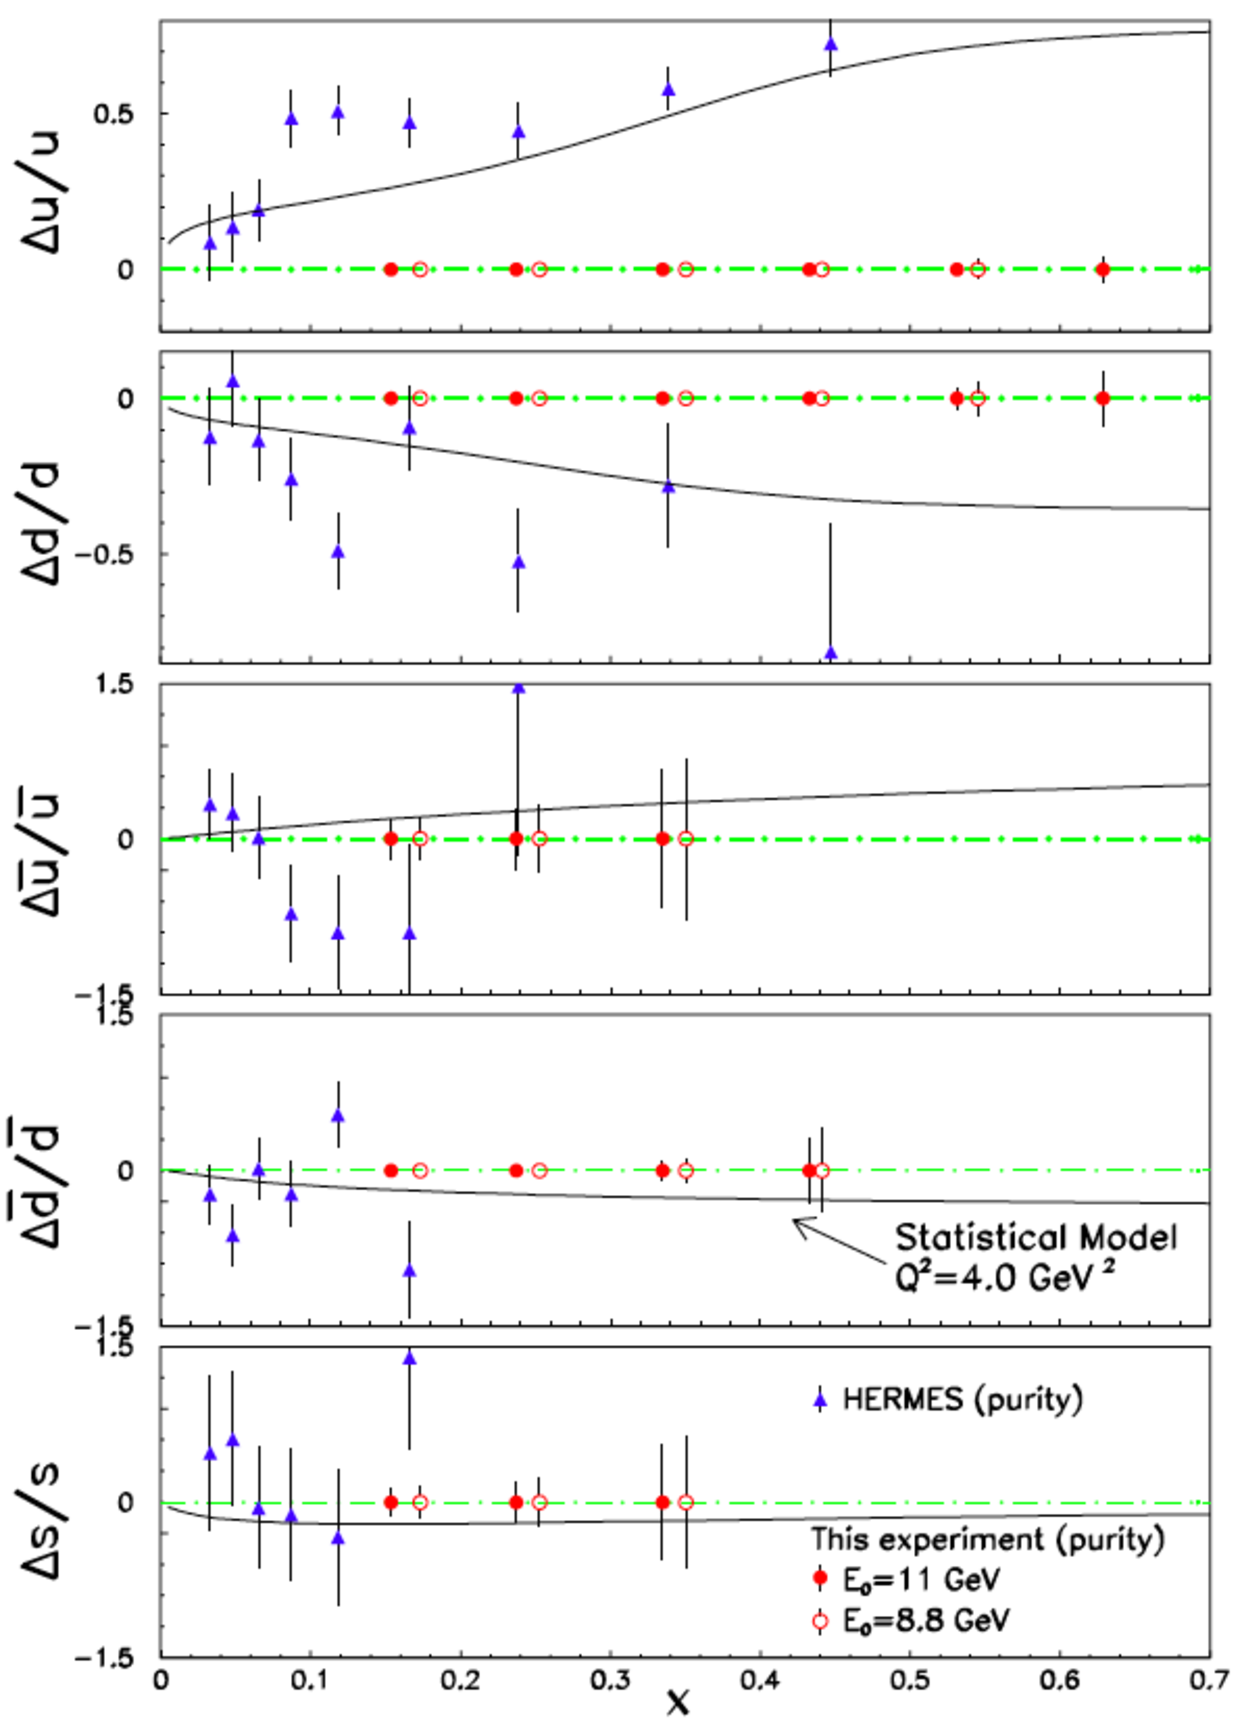
\includegraphics[width=0.92\linewidth]{figs_xj/delta5q_purity_060114.pdf}
\caption{\label{fig:delta5q} The expected statistical precision of $\Delta q/q$ from Leading Oder ``purity'' method.  
The published data of $\Delta q/q$ of  HERMES experiment~\cite{Airapetian:2004zf} are shown.  The COMPASS experiment~\cite{Alekseev:2010ub}  presented its results in $x\cdot \Delta q$ not in ratios.
Predictions of Statistical Model~\cite{Bourrely200739}, calculated at $Q^2=4.0$ GeV$^2$  are also shown.
}
\end{figure}
%-------------------------------------------------------------------------------

\section{Expected results fromLeading-Order Christova-Leader method}
\subsection{Statistical uncertainties of the combined asymmetries  $A_{1He}^{\pi^+ - \pi^-}$ }
The combined asymmetry $A_{1He}^{\pi^+ - \pi^-}$ needs the 
 cross section ratio $r=\sigma_{He}^{\pi^-}/\sigma_{He}^{\pi^+}$ as an extra input:
\begin{equation}
\label{Eq:obs2}
A_{1He}^{\pi^+ - \pi^-}  =  { \Delta \sigma_{He}^{\pi^+} -\Delta \sigma_{He}^{\pi^-} \over
\sigma_{He}^{\pi^+} - \sigma_{He}^{\pi^-} }=
{ A_{1He}^{\pi^+} -  A_{1He}^{\pi^-} \cdot r
\over 1 - r }.
\end{equation}
For this experiment, we have roughly $r=\sigma^{\pi^-}_{He}/\sigma^{\pi^+}_{He}=0.4 \sim 0.8$. 
The error propagation follows:
\begin{equation}
\label{Eq:errobs2}
(\delta A_{1He}^{\pi^+ - \pi^-})^2  = {1 \over (1 - r)^2} \left[ (\delta  A_{1He}^{\pi^+} )^2 + 
r^2 (\delta  A_{1He}^{\pi^-} )^2
+(A_{1He}^{\pi^+} - A_{1He}^{\pi^-} )^2   \cdot {(\delta r)^2  \over (1 - r)^2}  \right].
\end{equation}
The value of $r$ can be reasonably determined to better than 
 $|\delta r|/r \le 2.0 \%$  relatively in this experiment since phase spaces are identical for $\pi^+$ and 
$\pi^-$ measurements.  
 Inside the bracket of Eq.~\ref{Eq:errobs2}, the first term is always larger than the second term, while the third term is in the order of $(0.5\sim 1.5 \times10^{-3})^2$. 
Therefore, the first term dominates in Eq.~\ref{Eq:errobs2}, except in the few very high statistics bins at low-$x$ and low-$z$ in which  $A_{1He}^{\pi^+}$ can be  determined to better than $10^{-3}$. Basically, through Eq.~\ref{Eq:errobs2}, statistical uncertainties of $A_{1He}^{\pi^+ - \pi^-}$ receives an amplification factor  of $1/(1-r)$.

\subsection{Valence quark polarization}
Following Eq.~\ref{Eq:cl2},  we have  statistical uncertainties:
\begin{eqnarray}
\label{Eq:errcl2}
%&(\Delta u_v)_{LO}&  = {1 \over 5} \left[ \left( 4u_v - d_v)\cdot  A_{1p}^{\pi^+ - \pi^-}
%                 + (u_v + d_v) \cdot A_{1d}^{\pi^+ - \pi^-} \right) \right],  \\
& \delta \left( \Delta d_v-{1 \over 4} \Delta u_v  \right)_{LO} &  = {1 \over 4} \left( 7 u_v + 2 d_v \right)  \delta \left(A_{1He}^{\pi^+ - \pi^-} \right).
\end{eqnarray}

Statistical uncertainties of $\Delta d_v-{1 \over 4} \Delta u_v$, according to the Leading-Order Christova-Leader spin-flavor decomposition method and taking into account of effective neutron polarization in a $^3$He nuclei, are listed in Appendix~\ref{App:spin_flavor}, for each bin of $(x, Q^2, z)$, together with the expected statistical uncertainties in determining  $A_{1He}^{\pi^+ - \pi^-}$. For most bins of $(x, Q^2, z)$, the combined asymmetry $A_{1He}^{\pi^+ - \pi^-}$ can be determined to better than $1\%$ level. The $z$-dependence behavior of  $A_{1He}^{\pi^+ - \pi^-}$ (and $A_{1He}^{\pi^+ + \pi^-}$), for different $z$-bins corresponding to the same $(x,Q^2)$, can be used to verify the predicted Leading-Order $x-z$ naive separation, or set a systematic upper limit on how well this assumption holds. 

Once the $z$-dependence behavior is verified, data from different $z$-bins corresponding to the same $(x,Q^2)$ can be combined, the results are  listed in Table~\ref{tab:ddvallz}. 
Assuming other experiments  on polarized proton target can reach a similar  precision on  $\Delta u_v--{1 \over 4} \Delta d_v$,  especially from CLAS12 polarized NH$_3$ target SIDIS data,  the expected statistical uncertainties on $\Delta u_v -\Delta d_v$ 

%-------------------------------------------------------------------------------
\begin{table}[htbp]
\begin{center}
%\vspace{-0.5cm}
\begin{tabular}{|cc||c|c|c|}
\hline
$\langle x \rangle $   & $ \langle Q^2 \rangle $   & $\delta \left(A_{1He}^{\pi^+ - \pi^-} \right)$  &
$\delta \left[ x ( \Delta d_v -{1 \over 4} \Delta u_v ) \right]_{CL}$  & $\delta (\Delta u_v -\Delta d_v)_{CL}$ \\
                       & GeV$^2$              &  $\%$    &       &                                                       \\ \hline \hline
 E$_0$=11 GeV           &    5.20          &          &    &                                                                   \\ 
   0.166 &    3.29 &   0.25 &    0.0038 &    0.0259 \\
   0.249 &    4.64 &   0.18 &    0.0028 &    0.0125 \\
   0.347 &    6.09 &   0.22 &    0.0026 &    0.0084 \\
   0.445 &    7.38 &   0.30 &    0.0023 &    0.0058 \\
   0.532 &    8.65 &   0.46 &    0.0021 &    0.0045 \\
   0.629 &    9.65 &   0.83 &    0.0018 &    0.0032 \\
   0.720 &   10.73 &   2.16 &    0.0017 &    0.0027 \\ 
 E$_0$=8.8 GeV                      &       3.84       &          &    &                                                                 \\ 
   0.168 &    2.58 &   0.27 &    0.0042 &    0.0281 \\
   0.248 &    3.54 &   0.21 &    0.0032 &    0.0144 \\
   0.345 &    4.61 &   0.26 &    0.0032 &    0.0105 \\
   0.436 &    5.60 &   0.39 &    0.0033 &    0.0085 \\
   0.520 &    6.77 &   0.69 &    0.0036 &    0.0078 \\
   0.628 &    7.19 &   1.57 &    0.0037 &    0.0066 \\
   0.714 &    8.33 &  12.49 &    0.0117 &    0.0185 \\
\hline
\end{tabular}
\end{center}
\caption{\label{tab:ddvallz}  
Combining all $z$-bins for the same $(x,Q^2)$, the expected statistical uncertainties of   $A_{1He}^{\pi^+ - \pi^-}$ and  extracted valence quark polarization $\delta ( \Delta d_v -{1 \over 4} \Delta u_v )_{CL}$ according to leading order Christova-Leader (CL) method.  The expected statistical precision of $\Delta u_v -\Delta d_v$  are also listed, assuming other experiments  on polarized proton target can reach a similar  precision on $\Delta u_v$. 
}
\end{table}
%------------------------------------------------------------------------------
Statistical accuracies of $x \Delta d_v$ from this experiment, according to the
leading order Christova-Leader method, are plotted in Fig.~\ref{fig:xqvlo1}. Each data point represents a combination of six $z$-bins as listed in Appendix~\ref{App:spin_flavor}.
The published data from SMC~\cite{Adeva:1997qz}, 
HERMES~\cite{Airapetian:2004zf} and COMPASS~\cite{Alekseev:2010ub}, which used the ``purity'' method and included inclusive asymmetry data, are also plotted. Noticed that since the sum of $\Delta q+ \Delta \bar{q}$ is reasonably well-constrained by inclusive DIS data of spin structure functions $g_{1p}$ and $g_{1n}$, through SIDIS, statistical uncertainties on $\Delta q$ and $\Delta q_v$ follow as $\delta(\Delta q) \sim \delta(\Delta \bar{q})$ and   $\delta(\Delta q_v)=\delta(\Delta q-\Delta \bar{q}) \sim 2 \cdot \delta(\Delta \bar{q})$. 
QCD global fit of DSSV2008~\cite{DSSV2008} and a covariant Quark-Diquark Model~\cite{Cloet:2005pp} of I. Cloet {\it et al.} are also shown.
When the HERMES data were analyzed following the Christova-Leader method, dramatic increase
in statistical uncertainties can not be avoid due to the unfavorable cross section
ratio of $\sigma^{\pi^-}/ \sigma^{\pi^+}$ in the HERMES kinematics (see Fig.~\ref{fig:hermescl}
 in Appendix).  
 The SMC data, which assumed symmetric sea polarization, are also shown.  
%---------------------------------------------------------------------------------------------
\begin{figure}[htbp]
\centering
    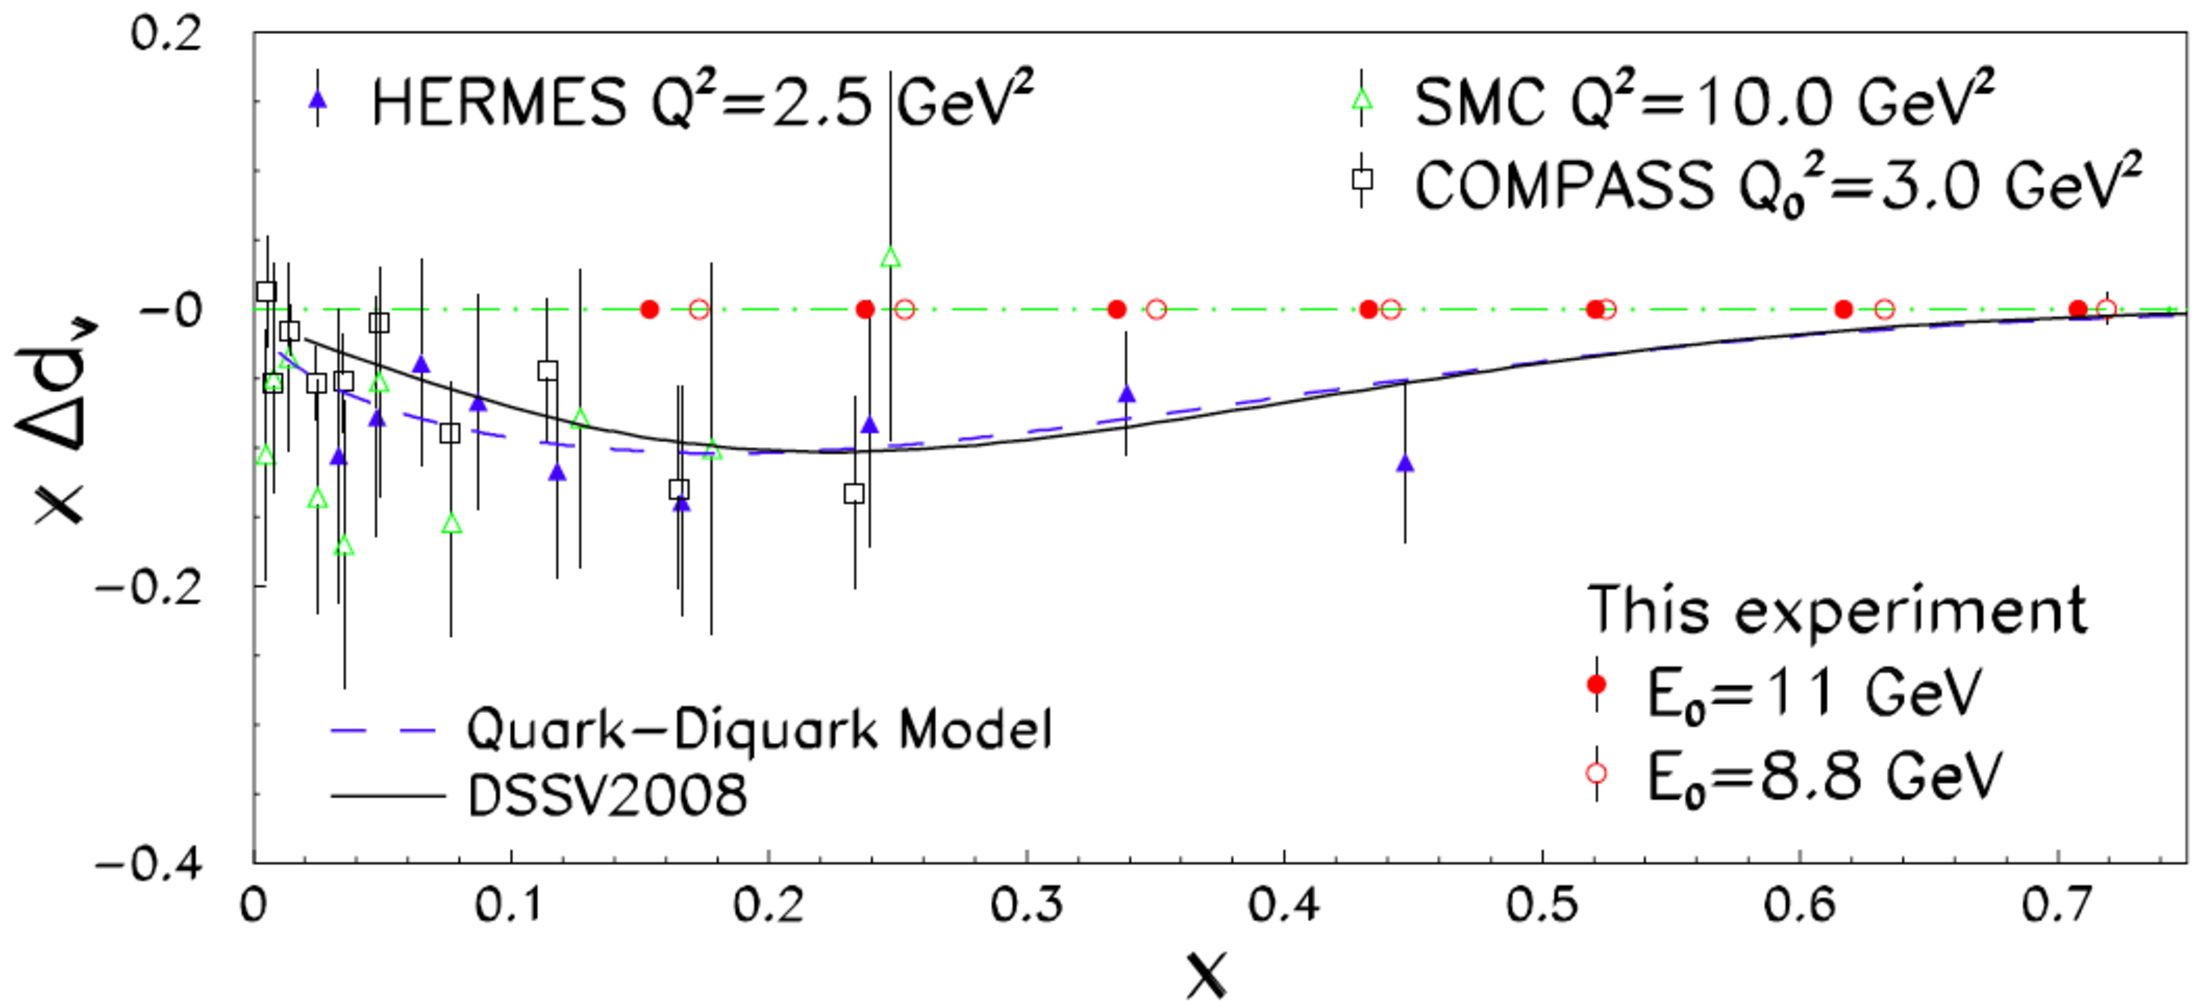
\includegraphics[width=0.98\linewidth]{figs_xj/xdeltadv_1pannel_052814.pdf}
\caption{\label{fig:xqvlo1} The expected statistical precision of $x \Delta d_v$ from Leading Oder Christova-Leader method.  Each data point represents a combination of six $z$-bins as listed in Appendix~\ref{App:spin_flavor}.
The published SMC~\cite{Adeva:1997qz}, HERMES~\cite{Airapetian:2004zf} and COMPASS~\cite{Alekseev:2010ub}  
 results which 
included a combined data set of inclusive and semi-inclusive asymmetries, are also shown. QCD global fit of DSSV2008~\cite{DSSV2008} and a covariant Quark-Diquark Model~\cite{Cloet:2005pp}, both calculated at $Q^2=4.0$ GeV$^2$,  are also shown.
}
\end{figure}
%-------------------------------------------------------------------------------


% list equations here.

When extracting $( \Delta d_v -{1 \over 4} \Delta u_v )_{LO}$ 
the knowledge of unpolarized PDF ($\delta q/q \approx \pm 4\%$)  contributes 
to the systematic uncertainties. Theoretical uncertainties  PDF on unpolarized  and $^3$He to neutron correction) dominate the systematics in $\Delta d_v$,  However, these systematic uncertainties are  to be multiplied by the size of  $A_{1He}^{\pi^+ - \pi^-}$, at the level of a few percent, when entering into $\Delta d_v$, % as listed in Table-\ref{tab:pdf}.

%Therefore, over the measured region, we have:
%\begin{equation}
 %\delta \left[ \int_{0.166}^{0.720}(\Delta d_v -{1 \over 4} \Delta u_v)dx \right]_{LO}  = \pm 0.023 ~(stat) \pm 0.025~(sys) ???
%\end{equation}
%Recall that from Eq.~\ref{Eq:bsr2}, if the moment of $\Delta d_v- \Delta u_v$ can be pinned down to $\pm$0.05, 
%the moment of polarized sea asymmetry can be constraint to $\delta \left[\int(\Delta \bar{u} - \Delta \bar{d})dx \right] = \pm 0.025$, eight
%standard deviations from the prediction of Chiral Quark soliton model.
% 
% This result on the valence quark moment is to be compared with the COMPASS deuteron results~\cite{compass2007} at $Q^2=10.0$ GeV$^2$:
%\begin{equation}
 % \left[\int_{0.006}^{0.7}(\Delta u_v + \Delta d_v)dx \right]_{LO} =  0.40 \pm 0.07 ~(stat) \pm 0.06~(sys) 
%\end{equation}


\subsection{Statistical uncertainty on $\Delta \bar{u} -\Delta \bar{d}$ when combined with JLab-12 GeV proton target data}
To further extract $\Delta \bar{u}-\Delta \bar{d}$ according to Eq.~\ref{Eq:cl4}, 
knowledge of $\Delta u_v - \Delta d_v$, and inclusive spin structure function  $g_{1p}$ and $g_{1n}$ are needed.  
Of course, the best option is to perform measurements on three different polarized 
targets (proton, deuteron and $^3$He) within the same experimental set up, such that
consistency checks are possible to set limits on systematic uncertainties of $\Delta u_v - \Delta d_v$.

For this experiment, we will follow the ``second best'' option.  The neutron ($^3$He) data from this experiment, or $\Delta d_v - {1 \over 4} \Delta u_v$,
will be combined with the world data on polarized proton target, especially from the planned CLAS12 measurement,
to obtain the best knowledge of $\Delta u_v - \Delta d_v$.

Assuming the world future proton target SIDIS data can reach the similar statistical uncertainties of this experiment,  and recall Eq.~\ref{Eq:cl4}:
\begin{eqnarray}
\left[\Delta \bar{u}(x) - \Delta \bar{d}(x) \right]_{LO} & = & 3 \left[ g_1^p(x)- g_1^n(x)) \right] 
 - {1 \over 2} (\Delta u_v - \Delta d_v) \vert_{LO}. \nonumber 
\end{eqnarray}
From JLab-6 GeV experiments~\cite{lit:bbfit,xiaochao}, currently  we have $\delta g_1^p \le 0.0059$, $\delta g_1^n \le 0.0057$.
Table~\ref{tab:pdfstat} lists the expected statistical uncertainties on $x(\Delta \bar{u}-\Delta \bar{d})_{LO}$, based on our current knowledge of $g_1^p(x, Q^2)$ and $g_1^n(x, Q^2)$.  We note that several  experiments at JLab-12 GeV,   such as the Hall A $A_{1n}$, Hall C $A_{1n}$  experiments, and CLAS12 measurements,  together with the BigBite single-arm electron measurement  of this experiment could dramatically reduce the uncertainties on the  inclusive spin structure  $g_1^p(x, Q^2)$ and $g_1^n(x, Q^2)$.
%-------------------------------------------------------------------------------
\begin{table}[h]
\begin{center}
%\vspace{-0.5cm}
\begin{tabular}{|cc|c|cc||c|}
\hline
$\langle x \rangle $ &  $\langle Q^2 \rangle $  & ${1 \over 2} \delta (\Delta u_v - \Delta d_v)$  & $3 \delta g_1^p$ & $3  \delta g_1^n$ & $\delta \left( \Delta \bar{u} - \Delta \bar{d} \right)_{LO}$  \\  \hline
       & & stat. & stat. & stat. & stat.  \\ 
  E$_0$=11 GeV &  5.20   &    &   &   &    \\
   0.166 &    3.29 &   0.0130 &  0.0177 &   0.0171 &    0.0278 \\
   0.249 &    4.64 &   0.0062 &  0.0177 &   0.0171 &    0.0254 \\
   0.347 &    6.09 &   0.0042 &  0.0177 &   0.0171 &    0.0250 \\
   0.445 &    7.38 &   0.0029 &  0.0177 &   0.0171 &    0.0248 \\
   0.532 &    8.65 &   0.0022 &  0.0177 &   0.0171 &    0.0247 \\
   0.629 &    9.65 &   0.0016 &  0.0177 &   0.0171 &    0.0247 \\
   0.720 &   10.73 &   0.0014 &  0.0177 &   0.0171 &    0.0246 \\
  E$_0$=8.8 GeV &   3.84  &    &   &   &    \\
    0.168 &    2.58 &   0.0141 &  0.0177 &   0.0171 &    0.0283 \\
   0.248 &    3.54 &   0.0072 &  0.0177 &   0.0171 &    0.0256 \\
   0.345 &    4.61 &   0.0052 &  0.0177 &   0.0171 &    0.0252 \\
   0.436 &    5.60 &   0.0042 &  0.0177 &   0.0171 &    0.0250 \\
   0.520 &    6.77 &   0.0039 &  0.0177 &   0.0171 &    0.0249 \\
   0.628 &    7.19 &   0.0033 &  0.0177 &   0.0171 &    0.0248 \\
   0.714 &    8.33 &   0.0093 &  0.0177 &   0.0171 &    0.0263 \\
\hline
\end{tabular}
\end{center}
\caption{\label{tab:pdfstat} Expected statistical uncertainties of  $(\Delta \bar{u} - \Delta \bar{d})_{LO}$, when combined with future SIDIS JLab-12 GeV proton target data,  taking  the current knowledge on inclusive DIS spin structure function $g_1^p(x, Q^2)$ and $g_1^n(x, Q^2)$.
}
\end{table}
%--------------------------------------------------------------------------------------------------------------------------------

 %---------------------------------------------------------------------------------------------
\begin{figure}[htb]
\centering
   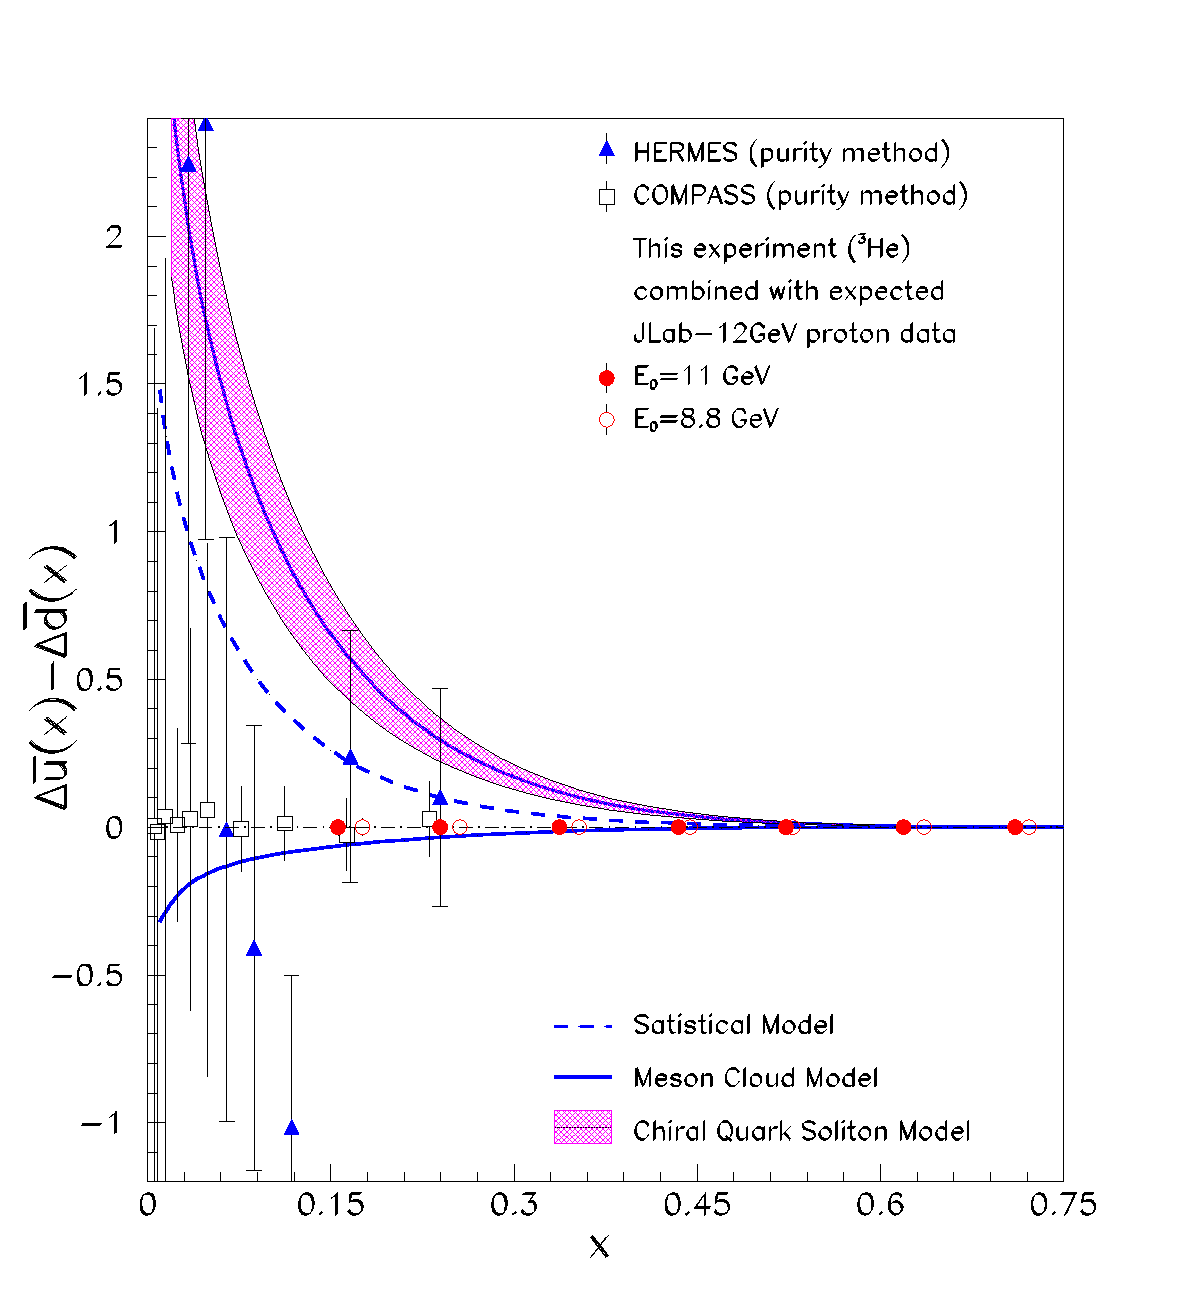
\includegraphics[width=0.8\linewidth]{figs_xj/polubdb_nox_053014.pdf}
\caption{\label{fig:dubdb1} 
The expected statistical accuracy of $\Delta \bar{u} - \Delta \bar{d}$, assuming JLab-12GeV proton target  data can reach a similar precision as this experiment. 
%Error propagation follows the HERMES 
%fragmentation function ratio. 
The published HERMES~\cite{Airapetian:2004zf} and COMPASS~\cite{Alekseev:2010ub}  purity 
results, which 
included combined data sets of inclusive and semi-inclusive asymmetries, are also shown.
Model predictions are from the Statistical Model~\protect\cite{Bourrely200739}, Meson Cloud Model~\protect\cite{cao} and 
the Chiral Quark Soliton
Model~\protect\cite{dressler}. 
}
\end{figure}
%-------------------------------------------------------------------------------

\section{Other systematic uncertainties}

\subsection{Effective nucleon polarization in $^3$He} \label{ch5:he3model}
Effective nucleon polarization in $^3$He for deep-inelastic scattering gives:
\begin{eqnarray}\label{equ:he3-g1n}
 g_1^{^3 {He}} &=& P_ng_1^n+2P_pg_1^p
\end{eqnarray}
where $P_n$($P_p$) is the effective polarization of the neutron 
(proton) inside $^3$He~\cite{theory:PnPp_friar}.
These effective nucleon polarizations $P_{n,p}$ can be
calculated using $^3$He wave functions constructed from N-N interactions,
and their uncertainties were estimated using various nuclear 
models~\cite{theory:PnPp_nogga,theory:PnPp_friar,theory:3Heconv,theory:PnPp_bissey},
giving 
\begin{eqnarray}
&& P_n=0.86^{+0.036}_{-0.02}~~{and}~P_p=-0.028^{+0.009}_{-0.004}~.\label{equ:PnPp}
\end{eqnarray}
%
The small proton effective polarization ($2.8 \%$) causes small 
offsets in the $^3$He asymmetries, compared to that from a 
free neutron.  The uncertainties associated with this small offset are even smaller
when considering that the corresponding proton asymmetries are better known
 and will be improved in the coming years.

At $x=0.110 \sim 0.461$, especially around $x=0.3$, the 
 nuclear EMC effect becomes rather small, as has been demonstrated 
on many different nucleus.

\subsection{$\pi$-$N$ final state interaction }
Since pions carry no spin,  $\pi N$ final state interactions will not introduce 
asymmetries in $A_{1He}^h$. Effect of $\pi$-$N$ final state interaction
will come through the dilution factors. By measuring the leading pions at
$4.3$ GeV/c, where the $\pi$-$N$ total cross sections are reasonably flat, 
effects of FSI are minimized. A detailed $\pi$-$N$ re-scattering calculation~\cite{misak}
confirmed that the modifications to the cross section are rather small at this kinematics.
 

\subsection{Target fragmentation and vector meson production }
 In principle, intermediate $\rho$ production processes are part
 of the fragmentation process and should not be subtracted
 from the SIDIS cross sections. Furthermore, 
 due to the charge conjugation, the effect of intermediate
 $\rho^0$ production is canceled in observables related to
 $\pi^+ - \pi^-$. Therefore, the Christova-Leader method of flavor decomposition
 is not sensitive to $\rho$ production.  
%Calculations of the yield of $(e,e^{\prime}\pi)$  from intermediate $\rho$ production
%have been done in the same Monte Carlo used for SIDIS reaction. The cross
%section for $N(e,e^{\prime}\rho^{\circ})X$ was calculated from a 
%modified version of the formalism used in PYTHIA \cite{Gaskell04}.

 At a high-$z$ setting of this experiment ($z \approx 0.5$), target fragmentation contamination is 
expected to be small, as has been shown by the HERMES LUND based Monte Carlo simulation. In addition, in the
$\pi^+ - \pi^-$ yield target fragmentation contributions are mostly canceled.


\subsection{Corrections from non-vanishing $A^n_{\perp}$ (or $A^n_{LT}$) }   
Since the target polarization is along the beam direction, not exactly along the
virtual photon  direction $\theta_{\gamma^{\star}}$, measurements of
$A_{\parallel}$ should in principle be corrected by a small contribution from $A_{\perp}$
in order to obtain the physics asymmetry $A_{1N}^h$.  
In this experiment, we have  $\sin \theta_{\gamma^{\star}} \approx 0.1$, therefore,
the uncertainty associated with this correction is of the order $0.1 \times (\delta A^n_{\perp})$. 

In the published HERMES and SMC data, the corrections from $A_{\perp}$ were neglected based on
the observation that in inclusive DIS $g_2(x)$ turned out to be rather small.  The residual
effect of non-vanishing $g_2$ (or $A_{\perp}$) in SIDIS has been included in the 
estimation of systematic uncertainties in the HERMES case. The contribution to the fractional 
systematic uncertainties on $A_{1N}^h$ was estimated to be $0.6 \%$ for proton and 
$1.4 \%$ for deuteron.

%In principle, about $10 \%$ of beam time of this experiment should be allocated
%for transverse target runs such that the exact corrections of $A^n_{\perp}$
%can be applied.  However, we chose not to request this extra beam time based
%on the following considerations:

\begin{itemize}
    \item  The leading order contribution in $A_{\perp}$ (or $A_{LT}$ in Mulders' notation)  
           is modulated by an angular dependence of $ \cos(\phi_s - \phi_h)$.
           When a reasonable range of $\phi_h$ is covered,  as in this experiment, 
           the averaged contribution from $A_{\perp}$ will most likely to be washed out.
 
    \item  Aside from the angular modulation, $A^n_{LT}$  was predicted to be at 
           the $10 \%$ level for the proton in bag-model calculations (Mulders, Yuan).
           Assuming $A^n_{LT}$ is at the similar level, the correction to $A_{1n}^h$
           will be at $1 \%$ level for this experiment, much less than the 
           statistical uncertainties.    
             
    \item  The value of $A^n_{LT}$ has been determined in the Hall A Neutron
           Transversity experiment~\cite{E06010_ALT_PRL}, with a in-plane transversely polarized $^3$He target, have provide
            information on $A^n_{LT}$.    Although $A_{LT}$ turned out to be non-zero,  its size is not large~\cite{E06010_ALT_PRL}
            In addition the transverse target run in SBS Transversity will also measure $A^n_{LT}$ to a high precision.
%            Although, $A_{\perp}$ turned out to be non-zero in E06-010, we will spend a few days of beam time 
%           HERMES experiment has already collected data on a transversely polarized
%           proton target with polarized positron beam, from which the  
%           beam-target double-spin asymmetry $A^p_{\perp}$ 
%           can be extracted. $A^n_{\perp}$ is expected to be much smaller than $A^p_{\perp}$.  
\end{itemize}  


